This chapter starts with exposing some problems with the existing specifications of the model. 
The latter part is our declarative specification of the model. 
We start by introducing \textit{agents} and \textit{event sets}, followed by various \textit{binary relations} defined between events. 
We then introduce certain helper definitions that prove useful in understanding the Axioms of the model. 
We then use the above elements to specify the \textit{axioms} of the model.
Lastly, we define \textit{races} followed by defining what a \textit{Consistent Execution} is as per the specification of the model.  
\ \newline
\ \newline  
\hrule 
\ \newline 
\ \newline 

\section{Elimination}

    Many programs which contain loops or are representing big softwares fall victim to having many redundant code. 
    This could also be possible due to differnt phases of optimization the compiler performs, which leaves certain residual code in each phase.
    One such example of redundant code is that when there are two consecutive reads or writes writing the same value to the same memory location.
    Another example could be the case that after many optimization passes, certain memory values are not used by the program itself, so the compiler may decide to remove it.  
    In a sequential setting the effect of removing such code is nothing.
    However, as we saw for simple reordering too, in a concurrent setting, elimination may not be that straightforward. 
    
    Let us for instance consider a program where we have two consecutive writes to the same memory writing the same value and the program after eliminating the latter write as below. 

    %SHow example here 

    
    The orange box shows the possible outcome that we want to consider. 
    In the first program, such an outcome should not be allowed. 
    While in the program after eliminating the latter write, this outcome is allowed.
    The following figure explains the relations formed in a candidate execution that can justify the observable behavior in question. 
    
    %Show relations here relevant

    The first set of relations is for the original program, where Axiom \ref{CoRe} prohibits the read $a$ to have value of $y$ as $2$.
    The second set is for the modified program, where none of the axioms.
    
    %For reads
    %I still do not have a counter example to show that elimination of reads is not safe. 
    %This is because I do not yet understand the implications of this on observable behaviors. 
    %Typically, if we remove the read from the set of observables, nothing should change, that is, restrictions on events agent ordered before or after the read must remain as it is.
    %This is because removal of restrictions might lead to new observable behaviors. 
    %The only case where this is not okay is when the read is part of a loop conditional. 
    %Removing such reads from every candidate will resort to non-termination of code.
    %One can jot this down to just restricting elimination of reads that are part of conditionals.
    %But otherwise, one can still eliminate. 
    %I am not sure which other case can be taken. How about showing when two reads are memory ordered without happens-before? Then elimination will not have any use.
    %We can skip this part for now and just refine the previous chapter first.
    An example where reads is unsafe to be eliminated is not quite easy to construct.
    This is because the semantics of the model does not really have any read-read dependance; one read value does not affect any subsequent(agent ordered) read value to same memory unless constrained by happens-before.
    So one might assume that we can freely eliminate reads: this however would not be safe to do, due to other reasons such as forward progress.
    If for instance, a loop repeatedly checks the value of some memory (say $x$) and will terminate only if the memory reads some fixed value, each candidate execution representing each iteration of the loop would represent also the minimum iterations before the read is of fixed value. 
    And this value would be of the read in the last iteration. 
    

    There are two types of elimination we are concerned with:
    \begin{itemize}
        \item Read Elimination
        \item Write Elimination
    \end{itemize}

    We address each part separately.


%AGENTS----------------------------------------------------------------------------------------------------------------------------------------  
\section{Agents}

    Agents represent threads in a concurrent program. As per the standard, they have more meaning than what we refer to here. However, with respect to the memory consistency model, we can safely abstract them to just represent threads/processes.

    \paragraph{Agent Cluster}
        Collection of agents concurrently communicating with each other through means of shared memory form an agent cluster.  There can be multiple agent clusters. However, an agent can only belong to one agent cluster. Agents communicating through message passing do not belong in the same agent cluster. 

        For our purpose, we assume just one agent cluster having one shared memory. 

    \paragraph{Agent Event List $(ael)$}
        Every agent is mapped to a list of events. The list represents the order in which the events are evaluated operationally\footnotemark. We define $ael$ as a mapping of each agent to a list of events.
        
        \footnotetext{The standard refers this to be an Event List, but we find it a bit misleading as it does not signify a list for each agent. Hence we name it as Agent Event List.} 

        

            



%Events------------------------------------------------------------------
\section{Events}
        
    Agent execution is modelled in terms of events. An event is either an operation that involves (shared) memory access or that constrains the order of execution of multiple events.

    \subsection{Event Types}
    
        Given an agent cluster, an \textit{event set} \set{E} is a collection of all events from the agent event lists. This set is composed of mainly two distinct subsets as follows: 

        \begin{itemize}
            \item \textbf{Shared Memory (\set{SM}) Events}
                
                This set is composed of two sets of events; those that write to shared memory called Write events (\set{W}) and those that read from shared memory called Read events (\set{R}). Events that belong to both Write and Read events are called Read-Modify-Write. 
            
            \item \textbf{Synchronize (\set{S}) Events} 
                These events only restrict the ordering of execution of events by agents. For instance $lock$ and $unlock$ type of events can be categorized under Synchronize events. However, this is not stated in the specification\footnotemark. 
    
                \footnotetext{The features of $Lock$ and $Unlock$ events is actually not something given to the programmer to use in Javascript. They areused to implement the feature $wait$ and  $notify$ that the programmer can use which adhere to the semantics of $futexes$ inLinux. Hence, in the original standard of the model, the distinction between lock and unlock is not made, and it is simplystated as Synchronize Event.}
        \end{itemize}
        
        \begin{figure}[H]
            \centering 
            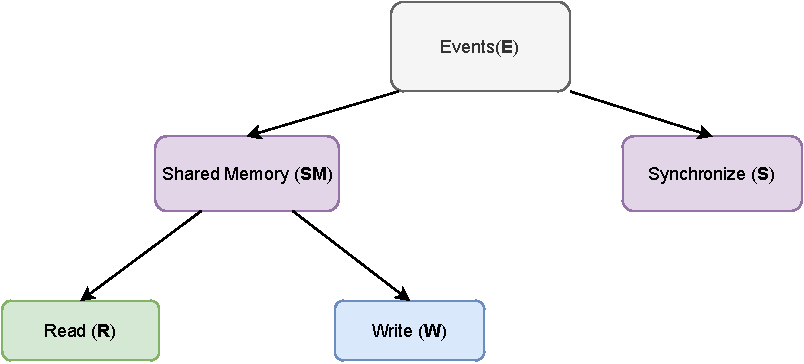
\includegraphics[scale=0.7]{4.ECMAScriptMemoryModel/EventTypes.pdf}
            \caption{The hierarchical categories of different sets of events.}
        \end{figure}

    %Range of events
    \subsection{Range ($\Re$)}
        Each of the \textit{shared memory events} are associated with a contiguous range of memory on which it operates. Range is afunction that maps a shared memory event to the range\footnotemark it operates on. This we represent as a starting index $i$ and a size$s$. So we could represent the range of a write event $w$ as 
                
                \[\Re(w) = (i, s) \]
    
        \footnotetext{The range as per the ECMAScript standard denotes only the set of contiguous byte indices. The starting byte indexis kept separate. We find this to be unnecessary. Hence we define range to have starting index and size.}
        
        We define the two binary operators below on ranges: 
        \begin{enumerate}
            \item Intersection $(\cap{_\Re})$ - Set of byte indices common to both ranges.
            \item Union $(\cup_\Re)$ - A unique set of byte indices that exist in both the ranges.  
        \end{enumerate}
        
        Two Ranges can be \textit{disjoint}, \textit{overlapping} or \textit{equal}. We use the binary operators to define these threepossibilities between ranges of events $e$ and $d$ :
        \begin{enumerate}
            \item Disjoint $\Re(e) \cap_\Re \Re(d) = \phi$ 
            \item Overlapping $(\Re(e)\cap_\Re \Re(d) \neq \phi) \wedge (\Re(e) \cap_\Re  \Re(d) \neq \Re(e) \cup_\Re \Re(d))$ - 
            \item Equal $\Re(e) \cap_\Re  \Re(d) = \Re(e) \cup_\Re \Re(d)$ - In simple terms, we define equality as $\Re(e) = \Re(d)$
        \end{enumerate}
            
%Types of Events Based on Order--------------------------------------------------------------------------------------------------------------------
    
    \subsection{Event Order / Event Access Mode} 
        Order signifies the sequence in which event actions are visible to different agents as well as the order in which they are executed by the agents themselves. In our context, there are mainly three types (in C11 memory model, they are called access modes) for each shared memory event that tells us the kind of ordering that it enforces. 
        
        \begin{enumerate}
            \item \textbf{Sequentially Consistent ($sc$)} - Events of this type are \textit{atomic}\footnotemark  in nature. There is a strict global total ordering of such events which is agreed upon by all agents in the agent cluster. 
            
            \item \textbf{Unordered ($uo$)} - Events of this type are considered \textit{non-atomic} and can occur in different orders for each concurrent process. There is no fixed global order respected by agents for such events. 
            
            \item \textbf{Initialize ($init$)} - Events of this type are used to initialize the values in memory before they are accessed by agent events. 
        \end{enumerate}

        All events of type \textit{init} are writes and all Read-Modify-Write events are of type \textit{sc}.  
        We represent the type of events in the memory consistency rules in the format ``$\textit{event} : \textit{type}$''. 
        When representing events in examples, the type would be represented as a subscript: $\textit{event}_\textit{type}$. 
       
        \begin{figure}[H]
            \centering
            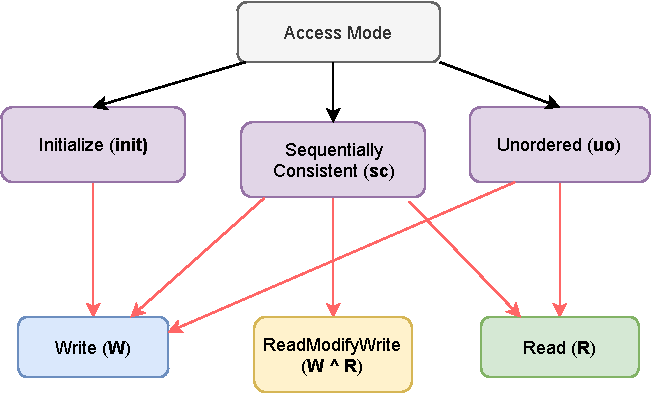
\includegraphics[scale=0.7]{4.ECMAScriptMemoryModel/AccessModes.pdf}
            \caption{Access Modes}
        \end{figure}

        \footnotetext{The word \textit{atomic} does not imply the events are evaluated using just one instruction. For example, a 64-bit sequentially consistent write on a 32-bit system has to be done with two subsequent memory actions. But its intermediate state of write must not be seen by any other agent. In an abstract sense, this event must appear '\textit{atomic}'.The \textit{atomic} here also refers to implications of whether an event's consequence is visible to all other agents in the same global total order or not. The compiler must ensure that for each specific target hardware, such guarantees are satisfied.}

%Tearing factor of events---------------------------------------------------------------------------------------------------------------------------

    \subsection{Tear Free ($tf$) or Tearing $!tf$)}
        Additionally, each shared-memory event is also associated with whether they are tear-free or not. OEvents that tear are non-aligned accesses requiring more than one memory access. Events that are tear-free are aligned and should appear to be serviced in one memory fetch\footnotemark.

        We represent the tearing of events in the memory consistency rules in the format ``$\textit{event} : \textit{tf/!tf}$''. 
        When representing events in examples, the type would be represented as a subscript: $\textit{event}_\textit{tf/!tf}$. 
       
        \footnotetext{It is not clear whether the alignment is with respect to specific hardware or not. The notion of one memory fetch may not be possible for all hardware practically, but it is something that must appear so. We will see a rule for ensuring this in the memory consistency rules.}
                       

%Relation among events----------------------------------------------------------------------------------------------------------------------------
    \section{Relation among events}
        We now describe a set of binary relations between events. These relations help us describe the consistency rules.
        
        \subsection{Read-Write event relations}
            There are two basic relations that assist us in reasoning about read and write events.

            %Read-bytes-from
            \paragraph{Read-Bytes-From $(\stck{_{rbf}})$}
            This relation maps every read event to a list of tuples consisting of write event and their corresponding byte index that is read. 
            For instance, consider a read event $e$ with range $(i, 3)$ and corresponding write events $d1$ and $d2$ with ranges $(i, 3)$ and $(i,4)$ respectively. 
            Possible $\stck{_\textit{rbf}}$ relations could be  
                \begin{align*}
                    \reln{e}{\textit{rbf}}{\{(d1, i), (d2, i\!+\!1), (d2, i\!+\!2)\}}. \\
                    \reln{e}{\textit{rbf}}{\{(d1, i), (d1, i\!+\!1), (d2, i\!+\!2)\}}. \\
                    \reln{e}{\textit{rbf}}{\{(d2, i), (d1, i\!+\!1), (d2, i\!+\!2)\}}.       
                \end{align*}   
            or having individual binary relation with each write-index pair as 
            \begin{align*}
                \reln{e}{rbf}{(d1, i)},\ \reln{e}{rbf}{(d2, i\!+\!1)}  \text{ and } \reln{e}{rbf}{(d2, i\!+\!2)}. \\
                \reln{e}{rbf}{(d1, i)},\ \reln{e}{rbf}{(d1, i\!+\!1)}  \text{ and } \reln{e}{rbf}{(d2, i\!+\!2)}. \\
                \reln{e}{rbf}{(d2, i)},\ \reln{e}{rbf}{(d1, i\!+\!1)}  \text{ and } \reln{e}{rbf}{(d2, i\!+\!2)}. 
            \end{align*}
            
            %Reads from relation
            \paragraph{Reads-From $(\stck{_{rf}})$}
            This relation, is similar to the above relation, except that the byte index details are not involved in the composite list. 
            So for the above examples, the \textit{rf} relation would be represented either as   
                $\reln{e}{rf}{(d1, d2)}$
            or individual binary read-write relation as 
                $\reln{e}{rf}{d1}$ and $\reln{e}{rf}{d2}$.
            Figure~\ref{model:read-from} below is an example of a program with its outcome (read values) shown in terms of reads-from relations.
            The left is a program example with the orange box representing one outcome of a program. 
            \begin{figure}[H]
                \centering
                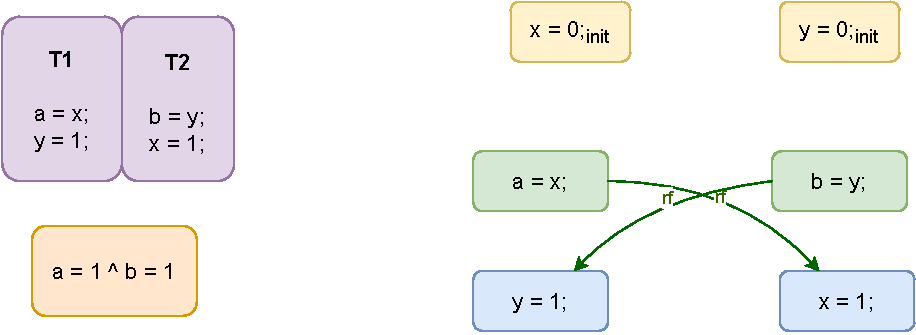
\includegraphics[scale=0.7]{3.ECMAScriptMemoryModel/ReadsFrom.pdf}
                \caption{An example showing \textit{reads-from} relations.}
                \label{model:read-from}
            \end{figure}
            
        %Agent sync with relation
        \subsection{Agent-Synchronizes-With (\set{ASW})}
            This is a set for each agent that consist of ordered tuples of synchronize events. 
            These tuples specify ordering constraints among agents at different points of execution. 
            So such a list for an agent $k$ would be represented like:  

                \[ASW_k = \{ \langle s1, s2 \rangle, \langle s3, s4 \rangle ...\}\]
        
            For every pair in the list, the first event ($s1$) belongs to the parent agent ($k$) and the second ($s2$) belongs to another agent it synchronized with\footnotemark.
                \[  
                    \langle s1, s2 \rangle \in ASW_k 
                    \Rightarrow{} 
                    s2 \notin ael(k).                        
                \]
            The ordered tuples are acyclic.
            \begin{align*}
                \langle s1, s2 \rangle \Rightarrow \neg \langle s2, s1 \rangle.
            \end{align*}

            Figure~\ref{model:agent-sync-with} below shows an example of this relation among two agents. 
            The left represents a program with synchronize events $s1$ and $s2$. 
            The orange box represents the synchronization established between the two agents.
            \begin{figure}[H]
                \centering
                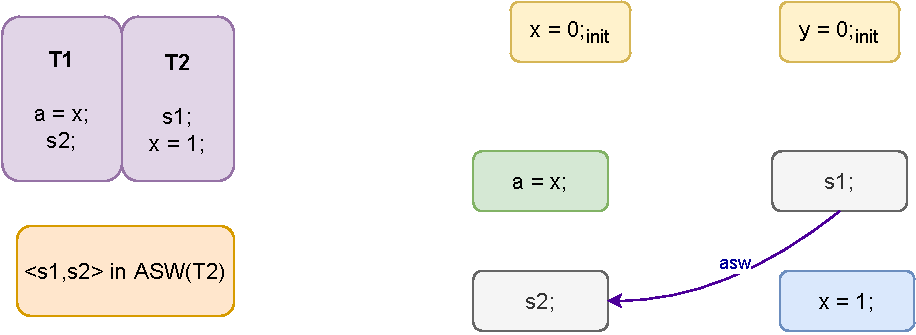
\includegraphics[scale=0.7]{3.ECMAScriptMemoryModel/AgentSyncWith.pdf}
                \caption{An example showing \textit{asw} relations.}
                \label{model:agent-sync-with}
            \end{figure}
        
        \footnotetext{This is analogous to the property that every unlock must be paired with a subsequent lock, which enforces the condition that a lock can be acquired only when it has been released.}

%Ordering Relation among Events----------------------------------------------------------------------------------------------------------------------       
\section{Ordering Relations among Events}
        
    We define agent-order, synchronize-with order, happens-before order and memory order using the binary relations defined on events in the previous section.
    %Agent Order
    \subsection{Agent Order ($\stck{_{ao}}$)}
        This is a union of the total orders among events belonging to the same agent event list. 
        It is analogous to \textit{intra-thread} ordering. 
        For example, if two events $e$ and $d$ belong to the same agent event list, then either $\reln{e}{ao}{d}$ or $\reln{d}{ao}{e}$. 
        Figure~\ref{model:agent-order} shows an example of agent order between events (right) composing a program (left).
        \begin{figure}[H]
            \centering
            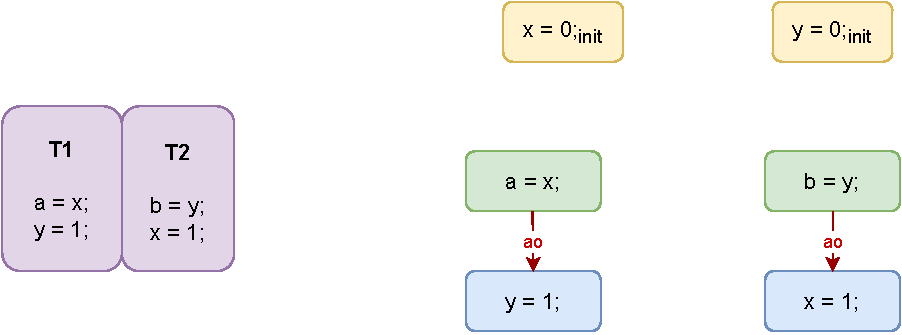
\includegraphics[scale=0.7]{3.ECMAScriptMemoryModel/AgentOrder.pdf}
            \caption{An example with \textit{agent-order} among events.}
            \label{model:agent-order}
        \end{figure}
    
    %Synchronize With Order
    \subsection{Synchronize-With Order ($\stck{_{sw}} $)}
        This is a binary relation between two events that establish synchronization between multiple agents. 
        It is a composition of two sets: 
        \begin{enumerate}
            \item All pairs belonging to $ASW$ of every agent belongs to this ordering relation. 
                \begin{align*}
                    \langle e_i, e_j \rangle \in ASW \Rightarrow{} \reln{e_i}{sw}{e_j}. 
                \end{align*}
                    
            \item The following reads-from pairs also belong to this ordering relation\footnotemark. 
                \begin{align*}
                    (\reln{r}{rf}{w}) \ \wedge \ \et{r}{sc} \ \wedge \ \et{w}{sc} \ \wedge \ (\Re(r)\!=\!\Re(w)) \ \Rightarrow{} \
                    (\reln{w}{sw}{r}).
                \end{align*}            
        \end{enumerate}
        Figure~\ref{model:sync-with} shows examples of such orders that can exist between events (right) of a program (left).
        The orange box represents the agent-synchronizes-with set that exists coupled with a possible outcome of the program (the final read value of $a$).
        \begin{figure}[H]
            \centering
            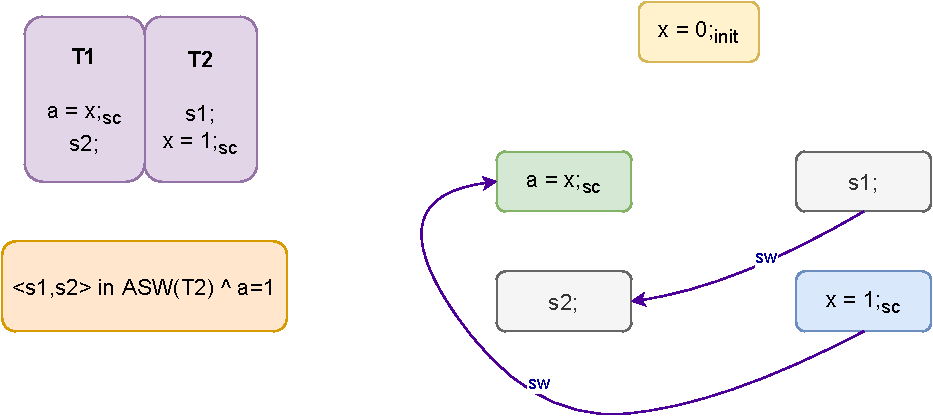
\includegraphics[scale=0.7]{3.ECMAScriptMemoryModel/SynchronizeWith.pdf}
            \caption{An example with \textit{synchronize-with} relations among events.}
            \label{model:sync-with}
        \end{figure}

        \footnotetext{Note that for the second condition, both ranges of events have to be equal. This however, does not mean that the read cannot read from multiple write events (refer the definition for $\stck{_{rbf}}$ in Subsection 3.3).}
        
    %Happens Before order 
    \subsection{Happens Before Order ($\stck{_{hb}}$)}
        This is a transitive order on events, composed of the following:
        \begin{enumerate}
            \item Every agent-ordered relation is also a happens-before relation 
                \begin{align*}
                    (\reln{e}{ao}{d}) \ \Rightarrow{} \ (\reln{e}{hb}{d}).    
                \end{align*}
                
            \item Every synchronize-with relation is also a happens-before relation 
                \begin{align*}
                    (\reln{e}{sw}{d}) \ \Rightarrow{} \ (\reln{e}{hb}{d}).    
                \end{align*}
                 
            \item Initialize type of events happen before all shared memory events that have overlapping or equal ranges between them. 
                \begin{align*}
                    \forall e,d \in SM \ \wedge \ 
                    \et{e}{init} \ \wedge \ 
                    (\Re(e) \cap \Re(d) \neq \phi)
                    \ \Rightarrow{} \ 
                    \reln{e}{hb}{d}.
                \end{align*}          
        \end{enumerate}
        Figure~\ref{model:happens-before} summarizes all possible patterns of happens-before order between events (right) of a program (left).
        The orange box, again represents the agent-synchronizes-with set that exists coupled with a possible outcome of the program (the final read value of $a$).
        \begin{figure}[H]
            \centering
            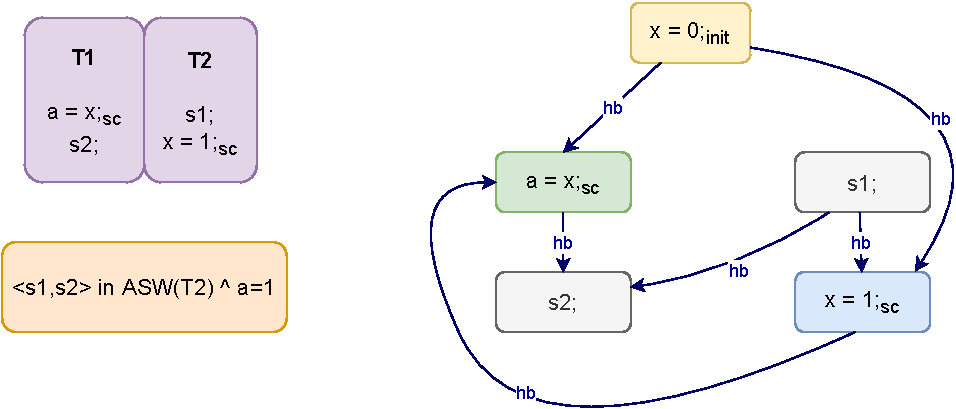
\includegraphics[scale=0.7]{3.ECMAScriptMemoryModel/Happens-before.pdf}
            \caption{An example with all the variants of \textit{happens-before} relations between events.}
            \label{model:happens-before}
        \end{figure}
    
    %Memory Order
    \subsection{Memory Order ($\stck{_{mo}}$)}
        This is a \textit{total order} on all events that respects happens-before order. 
        \begin{align*}
            \reln{e}{hb}{d} \Rightarrow{} \reln{e}{mo}{d}.    
        \end{align*}
        
        Figure~\ref{model:memory-order} is an example of a memory order between events (right) of a program (left).
        \begin{figure}[H]
            \centering
            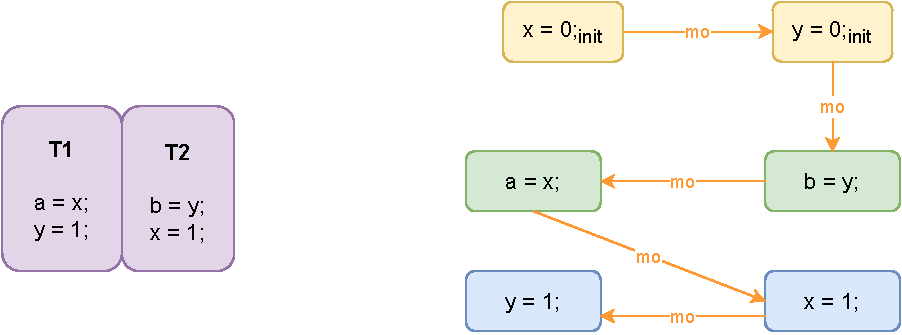
\includegraphics[scale=0.7]{3.ECMAScriptMemoryModel/MemoryOrder.pdf}
            \caption{An example with \textit{memory-order} (total) among all events.}
            \label{model:memory-order}
        \end{figure}


\section{Helper Definitions}
    
    Before we go into the consistency rules. we define certain preliminary definitions that create a separation based on a program, the axiomatic events and the various ordering relations defined above. This will help us understand where the consistency rules actually apply.    
    
    %What is a program 
    \begin{definition}{Program} 
        A \emph{program} is the source code without abstraction to a set of events and ordering relations. In our context, it is the original Javascript program. 
        
        %Note that here we need to supply a Javascript program using shared array buffers and atomic objects. A thing to do after we give examples for the ones below
    \end{definition}
    
%-----------------------------------------------------------------------------------------------------------------------------------------    
    %What is one run of a program to us?
    \begin{definition}{Candidate}
        A a collection of abstracted set of shared memory events of a program involved in one possible execution, with the $\stck{_\textit{ao}}$ relations. We can think of this as each thread having a set of shared memory events to run in a given intra-thread ordering. An example of a candidate is shown in figure~\ref{fig:candidate}.
        
        \begin{figure}[H]
            \centering
            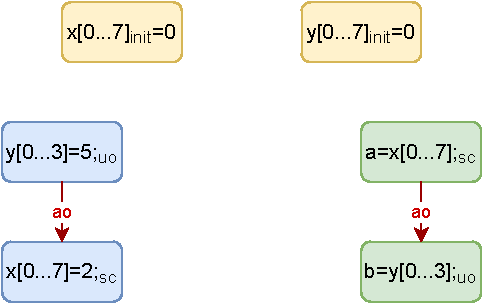
\includegraphics[scale=0.7]{4.ECMAScriptMemoryModel/candidate.pdf}
            \caption{An example of a Candidate}
            \label{fig:candidate}
        \end{figure}
        
    \end{definition}

%-----------------------------------------------------------------------------------------------------------------------------------------  
    \begin{definition}{Candidate Execution}
        A Candidate with the addition of $\stck{_\textit{sw}}$, $\stck{_\textit{hb}}$ and $\stck{_\textit{mo}}$ relations. This can be viewed as the witness/justification of an actual execution of a Program. Note that there can be many Candidate Executions for a given Candidate. The following figure shows an example of a candidate execution. 
        
        \begin{figure}[H]
            \centering
            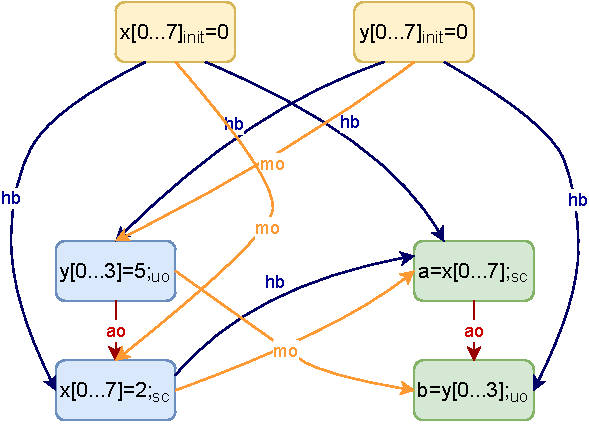
\includegraphics[scale=0.7]{4.ECMAScriptMemoryModel/CandidateExecution.pdf}
            \caption{An example of an Execution based on Candidate above}
            \label{fig:my_label}
        \end{figure}
        
    \end{definition}

 %-----------------------------------------------------------------------------------------------------------------------------------------   
    %What values are read when the program is run
    \begin{definition}{Observable Behavior}
    
        The set of pairwise $\stck{_\textit{rf}}$/$\stck{_\textit{rbf}}$ relations that result in one execution of the program. Think of this as our outcome of a program execution.
    
        \begin{figure}[H]
            \centering
            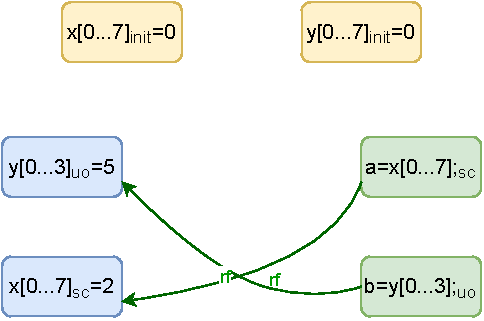
\includegraphics[scale=0.7]{4.ECMAScriptMemoryModel/Observables.pdf}
            \caption{Observable Behavior}
            \label{fig:my_label}
        \end{figure}
        
    \end{definition}

%-----------------------------------------------------------------------------------------------------------------------------------------
    
    \begin{definition}{Obs}
        We define $Obs_P, Obs_C, Obs_{CE}$ as functions that take a program, candidate and candidate execution respectively and give the set of observable behaviors possible by them. We are not concerned with the specific elements in this set, but the relation between the output of each of these functions among each other. 

        Consider a program $P$ whose candidates are $C_1, C_2, ... , C_n$. Consider for each candidate $C_i$, the candidate executions $CE_1, CE_2, ... CE_m$\footnotemark. Then, we have the following properties that hold:
        \begin{align*}
            Obs_P(P) = \cup_{i=1}^{n}Obs_C(C_i) \\ 
            Obs_C(C_i) = \cup_{j=1}^{m}Obs_C(CE_j)
        \end{align*}

        \footnotetext{Note that the variables $n$ and $m$ need not be finite.}
    \end{definition}

%-----------------------------------------------------------------------------------------------------------------------------------------
    

%Valid Execution Rules---------------------------------------------------------------------------------------------------------------------------------
        
    \section{Valid Execution Rules (the Axioms)}
        We now state the memory consistency rules. The rules are on \textit{Candidate Executions} which will place constraints on the possible \textit{Observable behaviors} that may result from it. 
         
%--------------------------------------------------------------------------------------------------------------------------------------  
        %Coherent Reads   
        \begin{axiom}{Coherent Reads} 
            \label{CoRe}
        
            There are certain restrictions of what a read event cannot see at different points of execution based on $\stck{_{hb}}$ relation with write events. 

            Consider a read event $e$ and a write event $d$ having at least overlapping ranges:
            \begin{align*}
                \event{e}{R} \ \wedge \ 
                \event{d}{W} \ \wedge \
                (\Re(e) \cap_\Re \Re(d) \neq \phi).
            \end{align*}

            \begin{itemize}
                %Rule #1
                \item A read value cannot come from a write that has happened after it 
                    \begin{align*}
                        \reln{e}{hb}{d}\ \Rightarrow{}\ \neg \ \reln{e}{rf}{d}.
                    \end{align*}
                    Figure~\ref{model:coherent_reads(1)} pictorially depicts the pattern above hwere $e$ cannot read from $d$.
                    \begin{figure}[H]
                        \centering
                        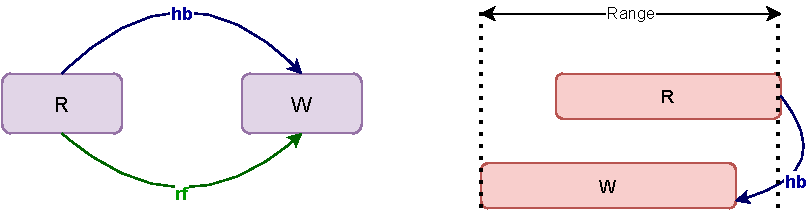
\includegraphics[scale=0.7]{4.ECMAScriptMemoryModel/CoherentReads1.pdf}
                        \caption{First axiom of Coherent Reads.}
                        \label{model:coherent_reads(1)}
                    \end{figure}
                %Rule #2    
                \item A read cannot read a specific byte address value from write if there is a write $g$ that happens between them which modifies the exact byte address. Note that this rule would be on the $rbf$ relation among two events. 
                    \begin{align*}
                        \reln{d}{hb}{e}
                        \ \wedge \ 
                        \reln{d}{hb}{g} \ \wedge \  \reln{g}{hb}{e}
                        \ \Rightarrow{} \
                        \forall x \in (\Re(d) \cap_\Re \Re(g) \cap_\Re \Re(e)), \ \neg \ \reln{e}{rbf}{(d,x)}.
                    \end{align*}
                    Figure~\ref{model:coherent_reads(2)} pictorially depicts the pattern where $e$ cannot read certain bytes from $d$. 
                    \begin{figure}[H]
                        \centering 
                        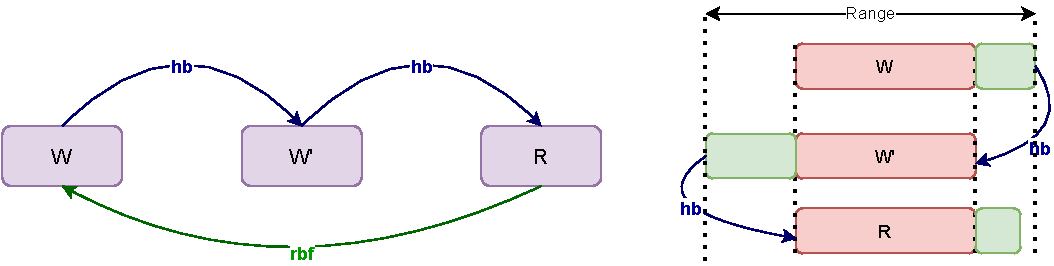
\includegraphics[scale=0.7]{4.ECMAScriptMemoryModel/CoherentReads2.pdf}
                        \caption{Second axiom of Coherent Reads.}
                        \label{model:coherent_reads(2)}
                    \end{figure}
                            
            \end{itemize}
        \end{axiom}
%------------------------------------------------------------------------------------------------------------------------------------------

        \begin{axiom}{Tear-Free Reads} 
            \label{TfRe}

            If two tear free writes $d$ and $g$ and a tear free read $e$ all with equal ranges exist, then $e$ can read only from one of them\footnotemark.
                
            \begin{align*}
                \et{d}{tf}\ \wedge\ \et{g}{tf} \ \wedge \ \et{e}{tf} 
                  \ \wedge \ 
                  (\Re(d) \!=\! \Re(g) \!=\! \Re(e)) 
                  \ \Rightarrow{} \\ 
                      ((\reln{e}{rf}{d}) 
                      \ \wedge \ 
                      (\neg \ \reln{e}{rf}{g})) 
                  \ \vee \  
                      ((\reln{e}{rf}{g}) 
                      \ \wedge \
                      (\neg \ \reln{e}{rf}{d})).
            \end{align*}
                    
            Figure~\ref{model:tear_free_reads(1)} shows the pattern that is disallowed among all tear-free events. 
            \begin{figure}[H]
                \centering
                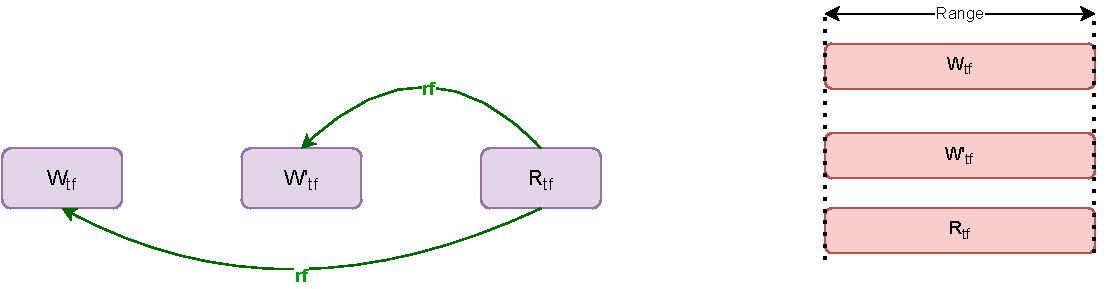
\includegraphics[scale=0.7]{4.ECMAScriptMemoryModel/TearFreeReads.pdf}
                \caption{Axiom of Tear-free reads.}
                \label{model:tear_free_reads}
            \end{figure}

            \footnotetext{To recap a tear-free event cannot be separated into multiple small events that do the same operation. However, considering different hardware architectures, the notion of tear-free need not necessarily mean this. (eg: A 64bit tear-free write to be done in a 32bit system). In a more abstract sense, we need an event to appear 'tear-free'.}    
        \end{axiom}

        \begin{axiom}{Sequentially Consistent Atomics}
            \label{SeqCsAt}   
            
            To specifically define how events that are sequentially consistent affects what values a read cannot see, we assume the following memory order among writes $d$ and $g$ and a read $e$ to be the premise for all the rules:  
                \begin{align*}
                    d \stck{_{mo}} g \stck{_{mo}} e.
                \end{align*}
               
            \begin{itemize}
                \item If all three events are of type $sc$ with equal ranges, then $e$ cannot read from $d$.
                    \begin{align*}
                        \et{d}{sc}\ \wedge\ \et{g}{sc}\ \wedge\ \et{e}{sc} 
                        \ \wedge \ (\Re(d) \!=\! \Re(g) \!=\! \Re(e))
                        \ \Rightarrow{} \ 
                        \neg \ \reln{e}{rf}{d}.
                    \end{align*} 
                        
                    Figure~\ref{model:sc_atomics(1)} depicts pictorially the pattern that is not allowed by this rule.
                    \begin{figure}[H]
                        \centering 
                        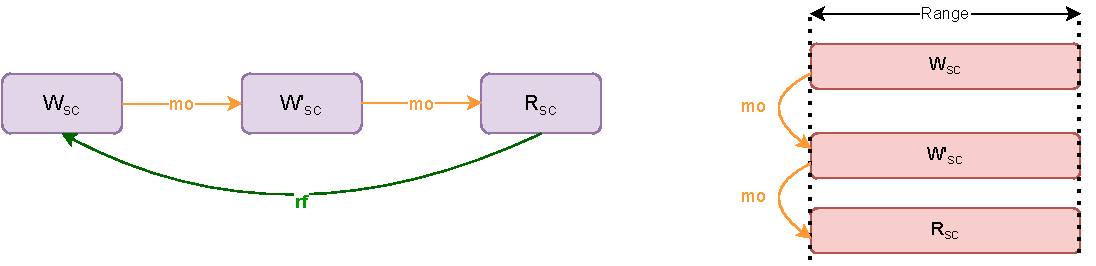
\includegraphics[scale=0.7]{4.ECMAScriptMemoryModel/SequentialAtomics1.pdf}
                        \caption{First Axiom of SC-Atomics.}
                        \label{model:sc_atomics(1)}
                    \end{figure}
                    
                \item If both writes are of type $sc$ having equal ranges and the read is bound to happen after them, then $e$ cannot read from $d$. 
                    \begin{align*}
                        \et{d}{sc}\ \wedge\ \et{g}{sc}  
                        \ \wedge \ (\Re(d) \!=\! \Re(g)) 
                        \ \wedge \ \reln{d}{hb}{e}
                        \ \wedge \ \reln{g}{hb}{e}
                        \ \Rightarrow{}\  
                        \neg \ \reln{e}{rf}{d}.
                    \end{align*}
                        
                    Figure~\ref{model:sc_atomics(2)} depicts pictorially the pattern that is not allowed by this rule.
                    \begin{figure}[H]
                        \centering 
                        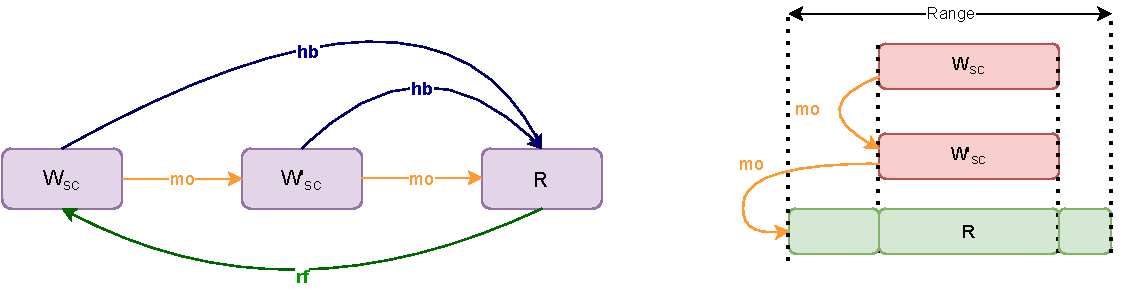
\includegraphics[scale=0.7]{4.ECMAScriptMemoryModel/SequentialAtomics2.pdf}
                        \caption{Second Axiom of SC-Atomics.}
                        \label{model:sc_atomics(2)}
                    \end{figure}
                
                \item If $g$ and $e$ are sequentially consistent, having equal ranges, and $d$ is bound to happen before them, then $e$ cannot read from $d$.
                    \begin{align*}
                        \et{g}{sc}\ \wedge\ \et{e}{sc}  
                        \ \wedge \ (\Re(g) \!= \!\Re(e)) 
                        \ \wedge \ \reln{d}{hb}{g} 
                        \ \wedge \ \reln{d}{hb}{e}
                        \ \Rightarrow \ 
                        \neg \ \reln{e}{rf}{d}.
                    \end{align*}

                    Figure~\ref{model:sc_atomics(3)} depicts pictorially the pattern that is not allowed by this rule.
                    \begin{figure}[H]
                        \centering 
                        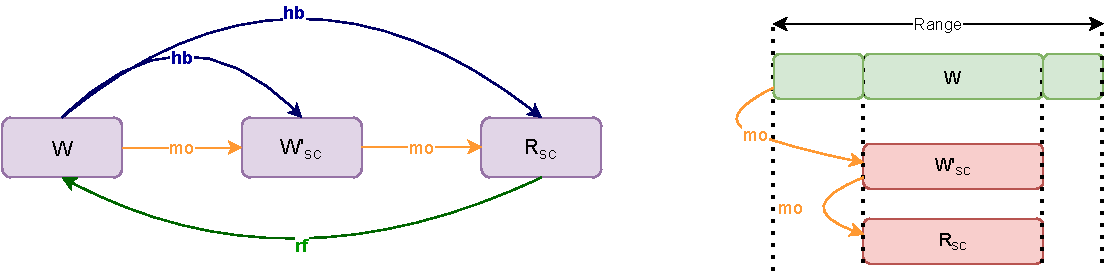
\includegraphics[scale=0.7]{4.ECMAScriptMemoryModel/SequentialAtomics3.pdf}
                        \caption{First Axiom of SC-Atomics.}
                        \label{model:sc_atomics(3)}
                    \end{figure}
                        
            \end{itemize}
        \end{axiom} 
        

%Races----------------------------------------------------------------------------------------------------------------------------------
        
    \section{Race}
        
        \subsection{Race Condition $RC$} 
            We define \set{RC} as the set of all pairs of events that are in a race. Two events $e$ and $d$ are in a race condition when they are shared memory events:
            \begin{align*}
                (e \in SM)\ \wedge\ (d \in SM).
            \end{align*}
            having overlapping ranges, not having a $\stck{_\textit{hb}}$ relation with each other, and which are either two writes or the two events are involved in a $\stck{_\textit{rf}}$ relation with each other. This can be stated concisely as,
            \begin{align*}
                \neg \ (\reln{e}{hb}{d})\ \wedge\ \neg \ (\reln{d}{hb}{e}) 
                \ \wedge \ 
                (
                (\event{e,d}{W}\  \wedge\ (\Re(d) \cap_{\Re} \Re(e) \neq \phi)) 
                    \  \vee\ (d \stck{_\textit{rf}} e)\ \vee\ (e \stck{_\textit{rf}} d)
                ).
            \end{align*}
                    
        \subsection{Data Race $DR$} 
            We define \set{DR} as the set of all pairs of events that are in a data-race. Two events are in a data race when they are already in a race condition and when the two events are not both of type \textit{sc}, or they have overlapping ranges. This is concisely stated as:  
            \begin{align*}
                \event{e,d}{RC}  \ \wedge \ 
                ((\neg\et{e}{sc} \ \vee \ \neg\et{d}{sc}) \ \vee \ 
                (\Re(e) \cap_{\Re} \Re(d) \neq \Re(e) \cup_{\Re} \Re(d))) 
            \end{align*}
            
            \critic{red}{The definition for data race also implies that sequentially consistent events with overlapping ranges are also in a data race. This may be counter-intuitive in the sense that all agents observe the same order in which these events happen.}
        
        \paragraph{Data-Race-Free (DRF) Programs}
            An execution is considered data-race free if none of the above conditions for data-races occur among events. A program is data-race free if all its executions are data race free.          
            \textit{The memory model guarantees Sequential Consistency for all data-race free programs (SC-DRF).}
        

%Consistent Executions-------------------------------------------------------------------------------------------------------------------

   %Consistent Executions-------------------------------------------------------------------------------------------------------------------

   \section{Consistent Executions (Valid Observables)}
      
      Consistent executions are those which should ideally be possible if the program is actually run on some hardware. 
      For a sequential program, we use the semantics of the programming language to understand what can be the outcome of a program. 
      For a concurrent program, since we can have multiple outcomes of the same program being executed (keeping all inputs constant), we need a semantic model to rely on. 
      The memory model is in essence just this semantic model for programs using shared memory.
      
      In our language, a consistent execution maps to a valid observable behavior, as this is what the user can actually record as an outcome of the program. 
   
      As per the standard specification, valid observable behaviour is when\footnotemark:
        \begin{enumerate}
           \item No $\stck{_\textit{rf}}$ relation violates the above memory consistency rules.
           \item $\stck{_\textit{hb}}$ is a strict partial order.
        \end{enumerate} 

        \textit{The memory model guarantees that every program must have at least one valid observable behaviour.}

        \footnotetext{There is also some conditions on host-specific events (which we mentioned is not of our main concern) and what is called a chosen read, which is nothing but the reads that the underlying hardware memory model allows. Since we are not concerned with the memory models of different hardware, this restriction on reads is not of our concern.}
    

\ \newline
\ \newline  
\hrule 
\ \newline 
\ \newline 
As a summary, this chapter axiomatically defined the ECMAScript memory model. 
We defined binary relations on events and specified the constraints of the model in terms of restricting reads-from relations that can exist between events in a Candidate Execution.
In the next chapter, we use this formal model to reason about the validity of instruction reordering.